\documentclass[12pt]{article}\usepackage[]{graphicx}\usepackage[]{color}\usepackage[]{subcaption}
%% maxwidth is the original width if it is less than linewidth
%% otherwise use linewidth (to make sure the graphics do not exceed the margin)
\makeatletter
\def\maxwidth{ %
  \ifdim\Gin@nat@width>\linewidth
    \linewidth
  \else
    \Gin@nat@width
  \fi
}
\makeatother

\definecolor{fgcolor}{rgb}{0.345, 0.345, 0.345}
\newcommand{\hlnum}[1]{\textcolor[rgb]{0.686,0.059,0.569}{#1}}%
\newcommand{\hlstr}[1]{\textcolor[rgb]{0.192,0.494,0.8}{#1}}%
\newcommand{\hlcom}[1]{\textcolor[rgb]{0.678,0.584,0.686}{\textit{#1}}}%
\newcommand{\hlopt}[1]{\textcolor[rgb]{0,0,0}{#1}}%
\newcommand{\hlstd}[1]{\textcolor[rgb]{0.345,0.345,0.345}{#1}}%
\newcommand{\hlkwa}[1]{\textcolor[rgb]{0.161,0.373,0.58}{\textbf{#1}}}%
\newcommand{\hlkwb}[1]{\textcolor[rgb]{0.69,0.353,0.396}{#1}}%
\newcommand{\hlkwc}[1]{\textcolor[rgb]{0.333,0.667,0.333}{#1}}%
\newcommand{\hlkwd}[1]{\textcolor[rgb]{0.737,0.353,0.396}{\textbf{#1}}}%
\let\hlipl\hlkwb

\usepackage{framed}
\makeatletter
\newenvironment{kframe}{%
 \def\at@end@of@kframe{}%
 \ifinner\ifhmode%
  \def\at@end@of@kframe{\end{minipage}}%
  \begin{minipage}{\columnwidth}%
 \fi\fi%
 \def\FrameCommand##1{\hskip\@totalleftmargin \hskip-\fboxsep
 \colorbox{shadecolor}{##1}\hskip-\fboxsep
     % There is no \\@totalrightmargin, so:
     \hskip-\linewidth \hskip-\@totalleftmargin \hskip\columnwidth}%
 \MakeFramed {\advance\hsize-\width
   \@totalleftmargin\z@ \linewidth\hsize
   \@setminipage}}%
 {\par\unskip\endMakeFramed%
 \at@end@of@kframe}
\makeatother

\definecolor{shadecolor}{rgb}{.97, .97, .97}
\definecolor{messagecolor}{rgb}{0, 0, 0}
\definecolor{warningcolor}{rgb}{1, 0, 1}
\definecolor{errorcolor}{rgb}{1, 0, 0}
\newenvironment{knitrout}{}{} % an empty environment to be redefined in TeX

\usepackage{alltt}
%\usepackage[english]{babel}
\usepackage[utf8]{inputenc}
\usepackage{amsmath}
\usepackage{graphicx}
\usepackage{setspace}
\usepackage[backend=bibtex]{biblatex}
\bibliography{references}
\usepackage{caption}
	  \usepackage{algorithm}
	  \usepackage{algpseudocode}

%\usepackage[square,sort,comma,numbers]{natbib}
\usepackage{url}
\usepackage{caption}
\usepackage{setspace}
\IfFileExists{upquote.sty}{\usepackage{upquote}}{}
\usepackage{listings}

\lstset{
	language=R,
	basicstyle=\ttfamily
}

\begin{document}

\begin{titlepage}
	\null
	\vspace{.5in}
	% Enter title here
	\begin{center}
		{\LARGE\bf My title...} \vspace{.1in}

		%{\LARGE\bf } \vspace{.1in}  \\

		%{\LARGE\bf } \vspace{.1in}  \\

		%{\LARGE\bf } \vspace{.1in}  \\

		%{\LARGE\bf } \vspace{.1in}  \\

		%{\LARGE\bf } \vspace{.1in}  \\


		\vspace{.05in}
		{\LARGE\bf $\;$} \\ [.5in]
		{\Large  Jordan R. Love \\
			\vspace{0.5cm}
			Department of Mathematical Sciences \\
			Montana State University \\ [.5in]}
		May 3, 2019 \\ [1.in]
		A writing project submitted in partial fulfillment\\
		of the requirements for the degree\\[.25in]
		Master of Science in Statistics
	\end{center}
\end{titlepage}

\begin{titlepage}
\null
\vspace{.5in}
\begin{center}
{\bf\huge APPROVAL}\\[1.in]
of a writing project submitted by\\[.25in]
Jordan R. Love \\[1.in]
\end{center}
\noindent
This writing project has been read by the writing project advisor and
has been found to be satisfactory regarding content, English usage,
format, citations, bibliographic style, and consistency, and is ready
for submission to the Statistics Faculty.

\vspace{.3in}
\begin{center}
\begin{tabular}{ll}
\rule{2.75in}{.03in} & \rule{2.75in}{.03in} \\
Date& Andrew B. Hoegh \\
& Writing Project Advisor \\
\end{tabular}
\end{center}

\vspace{1cm}

\begin{center}
\begin{tabular}{ll}
\rule{2.75in}{.03in} & \rule{2.75in}{.03in} \\
Date& Mark C. Greenwood \\
& Writing Projects Coordinator \\
\end{tabular}
\end{center}

\end{titlepage}

\newpage
\tableofcontents
\newpage

\begin{abstract}
Abstract goes here.
\end{abstract}

\doublespacing

\begin{document}

\maketitle

\section{Background \& Motivation}

As many organizations across a wide variety of fields begin to leverage larger amounts of data to understand and optimize their underlying processes, the role of statistical modeling becomes increasingly predictive and prescriptive, especially in professional sports. While the prediction of the outcomes of sports has always existed, more statistical approaches have only recently become more popular with the increased use of data in many sports. \cite{ruiz2015generative, dutta2017identifying} The rise of sabremetrics in baseball has acted as a catalyst for many other sports to begin accepting data-driven prediction and prescription \cite{chait_2004, roundtable_2013}. Sports betting alone has become a large political issue as large online fantasy sports sites such as DraftKings and FunDuel gained popularity \cite{rovell_2015}. Sports betting will remain a contentious issue for many states within the foreseeable futures, but the use of statistical models to enable and enhance these predictions will only increase. While this project does not focus on any professional sports league prediction or serious applications to betting, it does focus on a similar toy problem in order to learn more about the models and tools used in these areas.

The motivation for this project has three key aspects. The first is to learn about paired-comparison models and how they are used. paired-comparison models are employed to model the latent strength of either preferences within customers or performances of sports teams. The second aspect of this project is to explore the assumptions of connectivity required of the dataset. These requirements will be formulated in the language of graph theory to construct a comparison graph of the players within the dataset and matches played between them. Algorithms which can be used as a diagnostic for paired-comparison datasets are discussed, and a simulation related to the dataset analyzed in this project is summarized. The final motivating factor is to use models which integrate with existing decision optimization methods such as Markov decision processes. These will be described in more detail shortly. We will begin by describing the source of the dataset for this project: SaltyBet.

\subsection{What is SaltyBet?}

SaltyBet is an online, nonstop, ``Street Fighter'' game where A.I. driven characters fight against each other and human viewers are given fake ``Salty Bucks'' to bet on the outcome of each match \cite{kotaku}. SaltyBet is hosted on the Twitch platform, a popular video game streaming website where users can stream and commentate in real-time. SaltyBet was among the first to creatively use the platform to provide a unique viewer experience by making the entire stream automated. It has served as a forerunner in this style of stream automation with the even more popular stream ``Twitch Plays Pokemon'', citing SaltyBet as an inspiration \cite{hilliard}. An official launch date for SaltyBet cannot be verified. However, it has been running since at least April 26th, 2013 based on its accompanying Twitter account which tweets important match outcomes \cite{sbtwitter}. Since its inception, the Twitch stream has maintained a fairly consistent average of 400 users over the past year as reported by SullyGnome, a third-party Twitch platform statistics website. \cite{sullygnome}. A typical screen during a live match on SaltyBet.com is shown in Figure 1.

\begin{figure}[!h]
	    \centering
	    
\includegraphics[scale=0.15]{../images/SaltyBet.png}
	    \caption{Typical screen at SaltyBet.com of a match in progress -- The left vertical bar shows the users who have bet on the current match alongside their bet amount, the center vertical bar contains the match in progress and match odds, the right vertical bar shows the chat where users communicate.}
            \label{fig:my_label}
\end{figure}

Shortly after its inception, SaltyBet added a premium feature which allowed users to access all previous match data. This spawned the creation of many viewers opting to scrape and then use this data to build bots which automatically bet on match outcomes \cite{explosionduck, giantbomb}. These bots consist of many different types of algorithms. One of the more popular bots applies a genetic algorithm to rank and then predict the outcome of each match \cite{saltbot}. Among the bots reviewed for this project, none were found to apply a probabilistic approach to modeling each character's latent strength or incorporate other features of each character.

Within SaltyBet, each character consists of several features or traits which define the performance of the character. SaltyBet itself operates off of the MUGEN engine which was developed by ``elecbyte'' in early 2002 \cite{mugenwiki}. This engine clones the basic features of the classic Street Fighter series of games original developed by Capcom beginning in 1987 \cite{capcom_history}. The engine is designed with specifications to allow anyone to create custom characters. Since MUGEN's launch, a large number of characters have been created by the surrounding community. Of these created characters, 9,662 have fought at least one match on SaltyBet.com. The definition of each character must consist of a set of images which define the characters movement or ``moveset.'' A moveset describes all of the actions and motions a character can make to attack another character. The image used to define a character also defines its ``hitbox'': the area on the screen where a character can receive damage from other characters. Two example characters are shown in Figure 2. Notice specifically the large discrepancy in the hitbox height between the characters. Each character is also equipped with an AI script which defines how the character will attack and respond to other attacks. Finally, there are numeric values describing the attack strength, health, and meter (a measure of accessibility to highly effective attacks) associated with each character. Within the SaltyBet community, there exists a large number of hypotheses indicating discrepancies in the size of each character's hitbox can be predictive of match outcomes \cite{gamezone_2017}. An example of a hitbox discrepancy is shown in Figure 1. Generally, the character with the smaller hitbox (Figure 1b) has the advantage against the character with a large hitbox (Figure 1a). This is due to most attacks from the character shown in Figure 1a reaching over the hitbox of the character shown in Figure 1b while the opposite is not true. One goal of this project is to examine this ``hitbox advantage'' hypothesis in detail.

\begin{figure}[!h]
	\centering
	\begin{subfigure}[t]{.4\textwidth}
		\centering
		
\includegraphics{../images/jotaro-0.png}
		\caption{69 x 117 pixel hitbox}
		\label{fig:sub1}
	\end{subfigure}%
	\begin{subfigure}[t]{.4\textwidth}
		\centering
		
\includegraphics{../images/bwars-0.png}
		\caption{18 x 18 pixel hitbox}
		\label{fig:sub2}
	\end{subfigure}
  \caption{Example characters with their hitbox sizes listed as the number of pixels required to form the bounding rectangle}\label{fig:hitboxes}
\end{figure}


\subsection{Bayesian Methods}

In order to address the ``hitbox advantage'' hypothesis described previously, it is necessary to develop a probabilistic framework for evaluating the latent strength of characters and include additional information about the characters within the model. To do this, we will  use paired-comparison models. Specifically, a focus will be given to identifying hitbox advantages between characters through this model and determine at what level of hitbox differential advantages begin to arise. To do this, we will perform a brief review of paired-comparison Models and extensions for modeling additional information between characters.

It is of interest in this project to employ a Bayesian framework for a number of reasons. Bayesian methods often have large computational costs depending on the complexity of the model; however, there are also many advantages. The advantages relevant to this project are a natural estimation of variance, a recursive formula for online estimation, and integration in Markov decision processes.

\subsubsection{A Natural Estimation of Variance}

While it is beyond the scope of this project to detail the differences between frequentist and Bayesian methods, we will discuss specifically the advantage of estimation of variability. By natural estimation of variance, we are primarily referring to the lack of the need to apply higher order approximations (i.e. the Delta Rule) to compute variance of a transformation of random variables being modeled. One of the primary differences between Bayesian and frequentist methods is that the parameter under estimation is assumed to be random as opposed to fixed. Hence, a Bayesian modeling problem to can be interpreted, through use of Bayes' rule, in terms of probability distributions throughout. While not always trivial to obtain the resulting posterior distribution of a parameter within a complex model, all uncertainty for the parameter is contained within the samples of the posterior distribution. This includes variability which is a summary of the samples of the posterior distribution.

Within this and similar contexts, the interest is not only in predicting a point estimate describing which character or sports team is estimated to be most likely to win, but also quantifying our uncertainty around the estimate. This is not unlike financial markets where we are not only concerned with the overall performance but also the potential risk for large swings within the market due to uncertainty. Since one of the ideal applications of this model would be to form a ``trading strategy'', Bayesian modeling allows access to all necessary information to make an informed decision.

\subsubsection{A Recursive Formula}

Another advantage of Bayesian modeling is the recursive formula which can be formed by using the posteriors estimated at time $t-1$ as the prior distributions at time $t$. Many other statistical and machine learning techniques do allow this recursive estimation procedure to be implemented. Most notably, recursive least squares, an estimation technique found commonly in signal processing possesses a similar framework \cite{hayes_2014}. However, as with many other estimation techniques, Bayesian methods typically encompass a larger class of estimation procedures with specific prior choices being commonly known in literature simply as penalized methods (Regularized Least Squares, LASSO). Using Bayesian methods directly allows the penalization to come in the form of a prior distribution as opposed to a single term on the entire likelihood function. This is no different for recursive least squares with D.S.G. Pollock describing the relationship from a Bayesian perspective \cite{pollock}.

\subsubsection{Integration with Markov decision processes}

Markov decision processes (MDPs) are a formulation of the problem of the optimally moving around a space given some set of actions and known rewards. This optimization problem is often intractable to specify a priori due to the unknown rewards associated with each action and lack of observability of the entire system. This leads to a class of MDPs known as Partially Observable Markov decision processes (POMDPs) where the estimation of the current state of the system and optimal policy are estimated simultaneously. POMDPs are notoriously difficult to solve optimally, but the framework allows for many numerical methods to be applied for approximate optimal solutions to be found. This framework can be seen in many contexts such as air traffic control, surveillance, and robotics \cite{kochenderfer_2015}.

Since MDPs and POMDPs are both built on the theory of probability, Bayesian modeling provides a seamless integration into these methods for two reasons. The first is that we have a natural interpretation of variability in the language of probability constructed directly into our estimation procedure. The second is that the goal of both MDPs and POMDPs is typically not to make a single decision but to make multiple decisions over time. This allows the recursiveness of Bayesian methods again to seamlessly integrate with this process. For this reason, Bayesian methods are often the de-facto estimation procedures when dealing with these problems.

While implementing a POMDP is beyond the scope of this project, this framework was an important deciding factor in what model to choose to use as a natural extension from this project is to operationalize and optimize both which bets to make and how much to bet based on the information available.

\subsection{Structure of this Project}

This paper is divided into four primary sections. The first section describes the literature surrounding the Bradley-Terry variant of paired-comparison models. Separate sections describe various estimation techniques including maximum likelihood estimation and Bayesian estimation. The second primary section discusses the assumption of connectivity within paired-comparison models. In this section, we describe algorithms for determining if a dataset is sufficiently connected and what options are available if this assumption is not satisfied. In this section, we perform a graph-based simulation to determine the probability of connectivity within the dataset being analyzed in this project. In the third primary section, we perform three separate analyses using methods discussed in the model section and discuss their differences. We also describe all data collection procedures, data cleaning steps, and the results of the prediction of each of the three models fit on 500 additional matches. Finally, the concluding section concisely describes the results of the analysis and what future work may be performed to further the work of this project.

\section{Models}

Paired-comparison models were introduced formally in a statistical setting by Thurstone in 1927 \cite{thurstone_1927}. This paper introduced the ``Law of Comparative Judgement'' which is used in Psychometrics to measure test subject preferences. This was the first paired-comparison model formulated. The more developed model which we will focus on in this paper was first developed by Bradley and Terry in 1952 \cite{bradley_terry_1952}. The goal of a paired-comparison model is to model the probability of one item being chosen over another or the probability of one sports team defeating another. The quantities being estimated are latent preferences or strengths. The general goal of any paired-comparison model is to estimate parameters such that a model of the following form may be fit:

\[ P(A > B) = f(x) \]

Where $f(x)$ represents the paired-comparison model. In this project, we will focus on the Bradley-Terry formulation of paired-comparison models and discuss two additional variants beyond the basic model which allow for more information to be included within the model.

\subsection{Basic Bradley-Terry Model}

As previously described, paired-comparison models are interested in estimating the probability $P(A > B)$ where $A$ and $B$ are items or teams under comparison. The Bradley-Terry paired-comparison model formulates this problem in the following way:

\[ P(i > j) = \frac{\lambda_i}{\lambda_i + \lambda_j} \]

We have altered the indices from $A$ and $B$ to $i$ and $j$, respectively, to match the prevailing literature. This model similar to a logistic regression model. In fact, under the transformation $\lambda_i = e^{\pi_i}$, we obtain a function similar in form to a logistic regression. In fact, if the logit is taken of each side, a Bradley-Terry model can be interpreted as estimating contrasts between the estimated latent strength of the items being compared. This is the approach taken by Agresti which we will return to shortly. Using this formulation, we can derive the likelihood and log-likelihood functions for the Bradley-Terry model.

\begin{equation} \label{eq1}
\begin{split}
	L(\lambda_i) & = \underset{i \neq j}{\prod_{i=1}^{m}\prod_{j=1}^{m}} P(i > j) \\
	& = \underset{i \neq j}{\prod_{i=1}^{m}\prod_{j=1}^{m}} \bigg(\frac{\lambda_i}{\lambda_i + \lambda_j}\bigg)^{w_{ij}}
\end{split}
\end{equation}

Note that $w_{ij}$ represents the number of times $i$ has defeated or been chosen over $j$ and $m$ represents the total number of items. To derive the log-likelihood, first note the following useful definitions. First, we will define the total number of comparisons between $i$ and $j$ as $n_{ij}$ such that $n_{ij} = w_{ij} + w_{ji}$ and that $n_{ij} = n_{ji}$. Therefore, we have the following:

\begin{equation} \label{eq1}
\begin{split}
	\text{ln}L(\lambda_i) & = \underset{i \neq j}{\sum_{i=1}^{m}\sum_{j=1}^{m}} \text{ln}\bigg(\frac{\lambda_i}{\lambda_i + \lambda_j}\bigg)^{w_{ij}} \\
	& = \underset{i \neq j}{\sum_{i=1}^{m}\sum_{j=1}^{m}} w_{ij}\text{ln}(\lambda_i) - w_{ij}\text{ln}(\lambda_i + \lambda_j) \\
	& = \sum_{i=1}^{m} w_{i}\text{ln}(\lambda_i) - \underset{i \neq j}{\sum_{j=1}^{m}} w_{ij} \text{ln}(\lambda_i + \lambda_j)
\end{split}
\end{equation}

Using this model has several key assumptions. First, the outcomes are binary wins and losses or distinct choices between two options. There does exist modifications to Bradley-Terry models which permit ties, but those models will not be covered in this project. The interested read should see Davidson (1970) for more detail regarding this variant of the model. \cite{davidson1970} The second key assumption is that latent strengths do not change over time. For some sports modeling scenarios, this may or amy not be realistic. For SaltyBet, the characters participating are not adjusted once they have been added to the database. Therefore, this assumption has been met. One additional assumption is that there exists a suffucient number of connections within the dataset to estimate the comparisons of interest. This is covered in detail in Section 3 of this paper. Finally, we also assume for this model that no external factors affect the outcome besides the latent strengths being estimated. This may not always be the case as environmental factors may play a role in the outcome of choices or sports matches. This issue leads us to our next model variant.

\subsubsection{``Home-Field Advantage'' Model}

The ``home-field advantage'' variant of Bradley-Terry modls was originally developed by Agresti in his well-known text, Categorical Data Analysis \cite{agresti2011categorical}. As we mentioned previously, it is possible to view Bradley-Terry models as a specific formulation of logistic regression. It was in this context Agresti originally developed the additional effect to include a ``home-field advantage'' term in the model. This effect alters the probability statement of itnerest to a conditional statement depending on which team is currently playing at home. This effect can also be used to denote which character has a hitbox advantage by denoting the smaller hitbox character as having an ``advantage''. We will revisit the analysis of the dataset for this project using this formulation in Section 4. The altered probability statement is shown below.

\[P(i > j) = \left\{
    \begin{array}{lr}
    \frac{\theta\lambda_i}{\theta\lambda_i + \lambda_j} & : \text{if } i \text{ has the advantage}\\
		          \frac{\lambda_i}{\lambda_i + \theta\lambda_j} & : \text{if } j \text{ has the advantage}
			    \end{array}
			    \right.
			    \]

We can construct a likelihood function using a process similar to the basic model. Note that in this scenario, we will differentiate between wins made by $i$ against $j$ into those wins with an advantage as $w_{ij}^{+}$ and those made without an advantage as $w_{ij}^{-}$. Therefore, the likelihood function for this case becomes:

\begin{equation}
\begin{split}
L(\lambda_i) & = \prod_{i=1}^{m}\prod_{j=1}^{m} P(i > j) \\
 & = \prod_{i=1}^{m}\prod_{j=1}^{m} \bigg(\frac{\theta\lambda_i}{\theta\lambda_i + \lambda_j}\bigg)^{w_{ij}^{+}}\bigg(\frac{\lambda_i}{\lambda_i + \theta\lambda_j}\bigg)^{w_{ij}^{-}}
\end{split}
\end{equation}

In this case, we will make two additional defitions. First, that $w_i$ will represent the number of matches won by $i$ either advantaged or disadvantaged. We will also define $n^{+}$ as the total number of games won with an advantage. Using these definitions, we can derive a simplified log-likelihood expression.

\begin{equation}
\begin{split}
\text{ln}L(\lambda_i, \theta) & = \sum_{i=1}^{m}\sum_{j=1}^{m} \text{ln}\bigg(\bigg(\frac{\theta\lambda_i}{\theta\lambda_i + \lambda_j}\bigg)^{w_{ij}^{+}}\bigg(\frac{\lambda_i}{\lambda_i + \theta\lambda_j}\bigg)^{w_{ij}^{-}}\bigg) \\
& = \sum_{i=1}^{m} \sum_{j=1}^{m} \text{ln}\bigg(\frac{\theta\lambda_i}{\theta\lambda_i + \lambda_j}\bigg)^{w_{ij}^{+}} + \text{ln}\bigg(\frac{\lambda_i}{\lambda_i + \theta\lambda_j}\bigg)^{w_{ij}^{-}} \\
& = \sum_{i=1}^{m} \sum_{j=1}^{m} w_{ij}^{+}\text{ln}(\theta\lambda_i) - w_{ij}^{+}\text{ln}(\theta\lambda_i + \lambda_j) + w_{ij}^{-}\text{ln}(\lambda_i) - w_{ij}^{-}\text{ln}(\lambda_i + \theta\lambda_j) \\
& = \sum_{i=1}^{m} \sum_{j=1}^{m} w_{ij}^{+}\text{ln}(\theta) + w_{ij}^{+}\text{ln}(\lambda_i) - w_{ij}^{+}\text{ln}(\theta\lambda_i + \lambda_j) + w_{ij}^{-}\text{ln}(\lambda_i) - w_{ij}^{-}\text{ln}(\lambda_i + \theta\lambda_j) \\
& = n^{+}\text{ln}(\theta) + \sum_{i=1}^{m} \sum_{j=1}^{m} w_{ij}^{+}\text{ln}(\lambda_i) - w_{ij}^{+}\text{ln}(\theta\lambda_i + \lambda_j) + w_{ij}^{-}\text{ln}(\lambda_i) - w_{ij}^{-}\text{ln}(\lambda_i + \theta\lambda_j) \\
& = n^{+}\text{ln}(\theta) + \sum_{i=1}^{m} w_{i}\text{ln}(\lambda_i) + \sum_{i=1}^{m} xyz \\
\end{split}
\end{equation}

With this model, there are several potential downsides. The model forces each match to have an advantage associated with it. In the case of sports, there are many games which are played at neutral sites which do not have any advantage for either team. In the case of SaltyBet, there may only be advantages after a certain threshold of hitbox difference. In either case, it would be advantageous to have a model which allows us to incorporate an advantage only when plausible. It is beyond the scope of this project to determine a model which has three potential states for advantage, disadvantage, and neutral advantage. However, we discuss additional avenues for exploring these in the conclusion section of this project. We now turn our attention to the details of estimating the models discussed.
 
\subsection{Model Estimation}

\subsubsection{Maximum Likelihood Estimation}

The original algorithm for estimating probabilities of paired comparisons was developed before Thurstone formulated a model in full. Zermelo in 1929 developed and proved an algorithm which converged to a unique set of parameter estimates given certain conditions were met \cite{hunter2004mm}. These conditions are discussed more fully in section 3 as an analysis of the comparison graph. The algorithm described by Zermelo is outlined in algorithm 1.

\begin{algorithm}
\caption{Zermelo’s algorithm}\label{alg:zermelo}
\begin{algorithmic}[1]
	\Procedure{Zermelo}{$\lambda_i$}\Comment{Randomly initialized}
\State $r\gets a\bmod b$
\While{not converged or maximum iterations not reached}
    \State $\lambda_i^{(k)} \gets W_i\bigg(\sum_{i \neq j}^{m} \frac{N_{ij}}{\lambda_i^{(k-1)} + \lambda_j^{(k-1)}}\bigg)$
\EndWhile\label{euclidendwhile}
	\State \textbf{return} $\lambda_i$
\EndProcedure
\end{algorithmic}
\end{algorithm}

This procedure works by iteratively adjusting the latent strengths of each character depending on how many matches they have won (denoted by $W_i$) and by how many matches they have played against other characters (denoted as $N_{ij}$). This algorithm works as a basic maximum likelihood estimation optimization function where the parameters of interest are the latent strengths. This algorithm has convergence gaurentees which are discussed more throughly in Hunter \cite{hunter2004mm}. This algorithm does not extend to more general cases of the Bradley-Terry model such as ``home-field advantage'' models. For this, we will need to note a larger class of algorithms.

\subsubsection{Minorization-Maximization Algorithms}

While the algorithm described by Zermelo handles the most basic case, it was not extended to more advanced models such as the "home-field advantage" model. In this case, a more general theory of estimation algorithms surrounding Bradley-Terry models were developed. Lange, Hunter and Yang (2000) showed the algorithm developed by Zermelo is a specific case of a more general class of algorithms known as Minorization-Maximization (MM) Algorithms \cite{lange2000optimization}. One well known special case extending from this class of algorithms is the Expectation-Maximization (EM) Algorithm. Heiser (1995) describes in detail the connection between the MM and EM algorithms \cite{heiser1995convergent}.

Since the algorithm proved by Zermelo is a special case of MM algorithms, the estimation procedure only changes in notation between the original and latest literature. Hunter (2004) provides a detailed look at a large number of Minorization-Maximization algorithms. In the paper ``MM Algorithms for Generalized Bradley-Terry Models'', Hunter discusses extensions to the algorithm described previously to incorporate more efficient updating schemes. In addition, the primary focus is on extending the class of algorithm developed by Zermelo to more complex models accounting for both ``home-field advantage'' and allowing ties within matches. Due to the complexity of the algorithm, we will not discuss these algorithms in detail any further.

\subsubsection{Bayesian Estimation Methods}

While a review of classical statistical methods for estimating Bradley-Terry models have been review previously, the goal of this project is to develop a Bayesian view of Bradley-Terry models with the intent for these models to be used in conjunction with the mathematics of Markov decision processes. For this, we refer to the work of Caron and Doucet \cite{caron2012efficient}. Their paper ``Efficient Bayesian Inference for Generalized Bradley-Terry Models" describes the construction of Gibbs samplers for both the typical comparison and ``home-field advantage'' models through the reformulation of the likelihood function via different latent variables.

Classically, the latent variables of interest are the latent strength distributions which are denoted as $\lambda_i$ in the above discussion. The items of interest were then contrasts with a specific logistic regression where the coefficients are the latent strengths of each competitor. Instead of introducing this model, Caron and Doucet instead introduce the latent variable $Z_{i,j} = min(Y_{kj}, Y_{ki})$ where each $Y_kj, Y_{ki}$ is a realization from the underlying strength distribution of competitors indexed by $i$ and $j$, respectively. This allows the difference between two competitors to be captured in the new latent variable $Z_{i,j}$ as opposed to seperate latent variables $\lambda_i$ and $\lambda_j$. As is the case in other scenarios (Namely probit regression), inclusion of additional latent variables allows the model to be expressed in a sufficiently compact for to allow for Gibbs Sampling instead of requiring a more computational intensive Metropolis-Hasting algorithm for sampling. Using the latent variable formulation by Caron and Doucet, we introduce a Gibbs Sampler algorithm for each of the three model scenarios discussed above. We will not discuss the derivation of these models in detail but only setup the framework using key statements. More detailed derivations are found in the original paper by Caron and Doucet.

Caron and Doucet assume that the player peformance from each match is distributed as an exponential distribution with the rate parameter associated with each player describing the latent strength. The probability statement of interest is modified in a subtle but critical way for this context. Using an exponential distribution for each character, the match ups can be viewed as characters racing towards a finish line and a random sample from their associated exponential distributions are their arrival times. Therefore, if the ``performance'' output from a specific character during a match, $Y_{i,k}$, is less than its competitors, $Y_{j,k}$, character $i$ defeats character $j$ during match $k$. This is reflected as instead of the winning character having a larger value in the probability statement, a lower value than their competitor indicates success. 

Using the latent variable formulation discussed above, we can use well known results from mathematical statistics to note that the minimum of two exponential distributions is also distributed as an exponential distribution with the resulting rate parameter being the sum of the two rate parameters from the minimum \cite{casella2002statistical}. Now, since each character will ideally match up multiple times against a single character, we have that the latent variable $Z_{i,j}$ exists as the sum of all match results. Since each match result is distributed as an exponential distribution, we have the latent variable of interest $Z_{i,j}$ being distributed as a Gamma distribution with parameters $n_{ij}$ representing the number of matches between $i$ and $j$ and $\lambda_i + \lambda_j$ representing the distribution of the minimum of the two players strength distributions.

Finally, a prior distribution must be placed on the latent strength terms. Considering the case of comparing multiple characters, it is reasoanbly to assume that each prior must be identical for each character in order for the resulting inference to be fair \cite{twhelan2010}. Coran and Doucet define a prior for the latent strength of each character as a product of gamma distributions each having identical parameters $a$ and $b$ such that we have the following prior:

\[ p(\lambda) = \prod_{i=1}^{m} G(a, b) \]

Using these pieces, a Gibbs sampler is derived which consists of two steps shown in algorithm 2.

\begin{algorithm}
\caption{Basic Bradley-Terry Gibbs Sampler}\label{alg:basicbtgibbs}
\begin{algorithmic}[1]
	\Procedure{basicbt}{$\lambda_i$}
\While{maximum number of samples not met}
\For{$1 \leq < j \leq m$}
	\State sample $Z_{ij}^{(t)} | \lambda^{(t-1)} \sim G(n_{ij}, \lambda_i^{(t-1)} + \lambda_j^{(t-1)})$
\EndFor
	\For{i = 1, ..., $K$}
	\State sample $\lambda_i^{(t)} | Z^{(t)}\sim G(a+w_i, b+\sum_{i < j}Z_{ij}^{(t)}+\sum_{i > j}Z_{ji}^{(t)})$
	\EndFor
	\EndWhile\label{euclidendwhile}
\EndProcedure
\end{algorithmic}
\end{algorithm}

Per typical Gibbs sampling, we expect to see quick convergence using this method. Therefore, the maximum number of samples should be chosen and evaluated using typical measures of convergence such as visually inspecting trace plots or employing statistics such as the Gelman-Rubin statistic on the resulting posterior samples \cite{gelman1992inference}. Now, in order to account for ``home-field advantage'' a distribution must be placed on the advantage term, $\theta$. In the paper by Coran and Doucet, independent priors are placed on $\lambda$ and $\theta$ and $\theta$ is assumed to be distributed as a Gamma distribuion. Using this, we can again using a Gibbs Sampling approach to sample from this model as outlined in algorithm 3.


\begin{algorithm}
\caption{``Home-field advantage'' Bradley-Terry Gibbs Sampler}\label{alg:homebtgibbs}
\begin{algorithmic}[1]
	\Procedure{homebt}{$\lambda_i$}
\While{maximum number of samples not met}
\For{$1 < j \leq m$}
	\State sample $Z_{ij}^{(t)} | \lambda^{(t-1)} \sim G(n_{ij}, \theta^{(t-1)}\lambda_i^{(t-1)} + \lambda_j^{(t-1)})$
\EndFor
	\For{i = 1, ..., $m$}
	\State sample $\lambda_i^{(t)} | Z^{(t)}\sim G(a+w_i, b+\theta^{(t-1)}\sum_{i < j}Z_{ij}^{(t)}+\sum_{i > j}Z_{ji}^{(t)})$
	\EndFor
	\State sample $\theta^{(t)}| \lambda^{(t)}, Z^{(t)} \sim G(a_{\theta} + c, b_{\theta} + \sum_{i=1}^{K}\lambda_i^{(t)}\sum_{j\neq i}Z_{ij}^{(t)})$
	\EndWhile\label{euclidendwhile}
\EndProcedure
\end{algorithmic}
\end{algorithm}

While some modification is made to the strucuture of the Gibbs sampler, overall the typical requirements of the sampler remain the same. It will be necessary to seperate wins made with an advantage versus wins made without an advantage in order to efficiently use this programmatically. As described previously, typical convergence diagnostics are required in order to assess the success of the sampler. 

Now that we have covered both classical and Bayesian estimation methods for two key models which we will consider as part of this project, we will move into validating a key assumption of the dataset: connectivity.

\section{Comparison Graph Connectivity}

\subsection{Comparison Graph Definition}

One key assumption when using Bradley-Terry models for paired comparison modeling is the data is in such a format that the comparisons of interest can be estimated. In many cases when a paired-comparison model is employed, all or most items being compared have been compared to each other at least once and no item has been chosen over all other items in its comparisons. If we consider professional sports as an example, each team typically plays most other teams at least once and some teams multiple times. This leads to many connections among a comparatively small number of teams. The probability of the dataset being appropriate for paired-comparison modeling is high. However, within many college sports the number of teams is far larger than the number of matches any one team will play during a season. This leads to a much lower probability of the dataset containing a sufficient number of games between teams to be appropriate for paired-comparison modeling. We can validate the assumption through the use of graph theory.

A first principles view of graph theory is beyond the scope of this paper, but the author refers interested readers to Chartrand for a more detailed treatment \cite{chartrand_1977}. graph theory studies objects known as graphs which represent a generalized form of objects and relations. Graphs in this sense are not visualizations but a collection of ``nodes'' and ``edges''.  Nodes represent atomic items such as sports teams or choices where edges may represent matches between teams or preferences between choices. Edges represent the relationships between nodes. An intuitive example is that of a social network. Consider a group of people who each may or may not know each other. Each person would be represented as a node within this graph. We can places edges between nodes where there exists an acquaintance.

A graph can be an undirected or directed. In the case of an undirected graph, a single edge is placed between two nodes indicating a general relationship. In the case of our social network example, an undirected graph would be appropriate. Within an undirected graph, we can visualize moving between two nodes without restriction whenever any edge connects them. A directed graph adds an additional layer of information for direction. For the purposes of this project, the nodes under consideration are characters which have played at least one match on SaltyBet. Each directed edge between two characters indicates the outcome of a match where the direction will extend from the winning character to the defeated character. In the case of a directed graph, we can visualize movement between characters in the same way as an undirected graph, but our options are more restricted due to the additional layer of direction between characters.

The graph we have described represents a \textit{comparison graph}. This graph defines all matches played between characters as directed edges and will be used to assess the necessary assumptions of connectivity for paired-comparison modeling. Figure 3 shows two examples of connected and disconnected directed comparison graphs in Figure 3a and Figure 3b, respectively.

\begin{figure}[!ht]
	\centering
	\begin{subfigure}[t]{.45\textwidth}
		\centering
		\captionsetup{width=0.85\textwidth}
		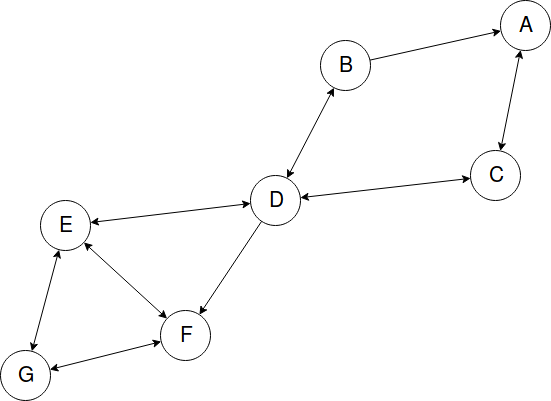
\includegraphics[scale=0.3]{../images/SampleConnectedGraph.png}
		\caption{This graph is strongly connected as there exists a path using directed edges between any two nodes in the graph.}
		\label{fig:sub1}
	\end{subfigure}%
	\begin{subfigure}[t]{.45\textwidth}
		\centering
		\captionsetup{width=0.85\textwidth}
		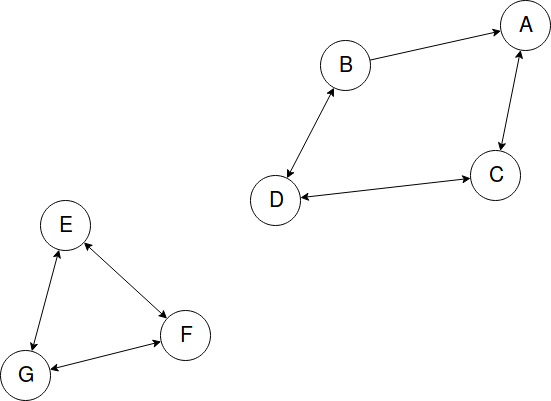
\includegraphics[scale=0.3]{../images/SampleDisconnectedGraph.png}
		\caption{This graph is entirely disconnected as there exists disjoint subsets of nodes which have no connections between them.}
		\label{fig:sub2}
	\end{subfigure}%
	\caption{An example of two comparison graphs with nodes A through G representing sample competitors.}\label{fig}
\end{figure}

\subsection{Condition of Strong Connectivity}

The original constraint for paired-comparison data to be suitable for analysis such that all comparisons can be estimated was formulated by Ford in 1957 \cite{ford_1957}. This requirement stipulated that the comparison graph must be such that any node within the graph can be chosen and directed edges exists in such a way that movement along the existing edges admits a path to any other node in the graph. In graph theoretic terms, this condition is equivalent to \textit{strong connectivity} or stating that the comparison graph has the property of being \textit{strongly connected}. It is important to note this is a stronger statement than an undirected graph being connected as the ``one-way streets'' formed by directed edges may not necessarily form a strongly connected graph. Figure 4a shows an example of a directed graph which has an edge between all nodes but is not strongly connected. We will revisit the relationship between strong connectivity and undirected graphs shortly.

In order to evaluate this assumption within a dataset of comparisons, we can use well known algorithms to determine the connectivity of the comparison graph. Tarjan's Algorithm \cite{tarjan_1972} by Robert Tarjan is an efficient algorithm which runs in linear time with regard to the number of nodes within a graph and determines the number of strongly connected components within a graph. Strongly connected components of a graph are disjoint subsets of nodes which are independently strongly connected despite the graph as a whole not being strongly connected. This algorithm can serve two purposes within the context of paired-comparison models. If the interest is in determining if the comparison graph is strongly connected, then the desired output from this algorithm is that the graph is constructed from one strongly connected component. However, in the event there exist more than one strongly-connected component within the graph (implying the entire graph is not strongly connected), the algorithm will return labels corresponding to disjoint sets of nodes which are strongly connected. In this case, a paired-comparison model can be fit to each of the strongly connected components identified, but comparisons across the strongly connected components will be unavailable. Figure 4a shows an example of a graph containing two strongly connected components while figure 3a shows an example of a graph being strongly connected.

\begin{figure}[!h]
	\centering
	\begin{subfigure}[t]{.45\textwidth}
		\centering
		\captionsetup{width=0.85\textwidth}
		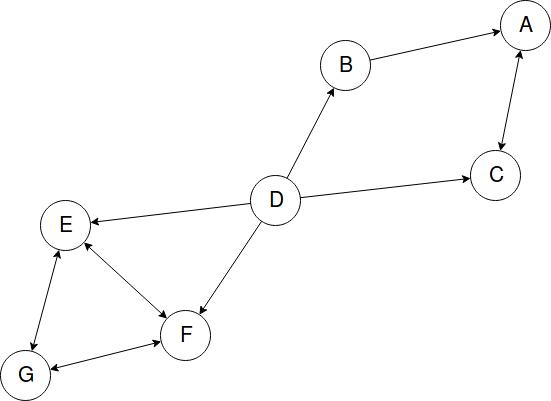
\includegraphics[scale=0.3]{../images/SampleWeaklyConnectedGraph.png}
		\caption{This graph is weakly connected as there does not exist a path along directed edges between all nodes in the graph.}
		\label{fig:sub1}
	\end{subfigure}%
	\begin{subfigure}[t]{.45\textwidth}
		\centering
		\captionsetup{width=0.85\textwidth}
		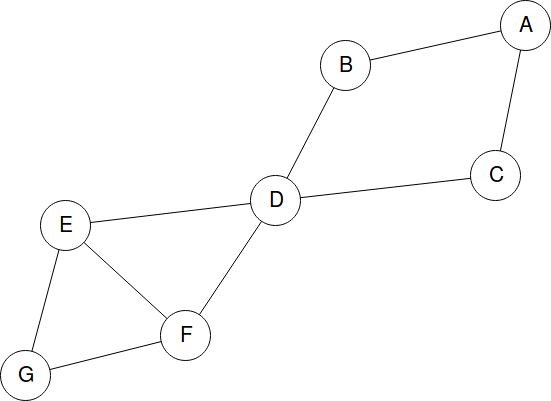
\includegraphics[scale=0.3]{../images/SampleUndirectedWeaklyConnectedGraph.png}
		\caption{This graph is weakly connected as it is a transformation of the graph shown in Ya where each directional edge is replaced with a undirected or bidirectional edge. Using this transformation, there exists a path between any two nodes in the graph implying weak connectivity of the graph shown in 4a.}
		\label{fig:sub2}
	\end{subfigure}%
	\caption{An example of comparison graphs representing weak connectivity in both a directed and undirected setting using nodes A through G as example competitors.}\label{fig}
\end{figure}

\subsection{Condition of Weak Connectivity}

While strong connectivity of the comparison graph allows a paired-comparison model to be fit without issue, Yan discusses how using a singular perturbation method can allow for comparisons to be made when the graph is only \textit{weakly connected} \cite{yan2016ranking}. Weakly connected graphs are directed graphs which, if transformed into an undirected graph and all directed edges are made undirected, the graph is connected (or all nodes can be reached from any other node). Figure 4a shows an example of a graph which is not strongly connected but is weakly connected. In Figure 4a, we see the original directed graph with node D having only directed edges away from it. However, if we remove the direction from each of the edges, we see in Figure 4b that the undirected version of this graph is connected. One intuitive reason for why weakly connected graphs are not sufficient without modification is that one team is undefeated and without an additional measure of ``strength of win'', the magnitude of how much the latent strength of this team differs from the next best team is unknown. Another intuitive reason is that node D in Figure 4a prevents the flow of information between strongly connected components.

The singular perturbation method discussed by Yan is equivalent to adding a penalized term to the likelihood in such a way that a ``pseudo-loss'' to at least one other team is added to the comparison graph in order for the graph to become strongly connected. This penalizer term can be re-interpreted as a specific prior distribution. Depending on the framework being employed, the prior distribution will differ. The next section reveals why this method was not required for large datasets, but can be adapted depending on the needs of the dataset.

\subsection{Simulation of Graph Connectivity}

It is useful to understand how likely a graph is to be connected given some properties (number of nodes, number of edges). Assessing the probability of a graph being connected is a difficult combinatorial problem to solve analytically. However, it is possible to simulate the connectedness of a graph. In the case of the data we are analyzing, we assume that two characters are randomly chosen to participate in a match. This is a strong assumption about the underlying structure of how characters are chosen for a given match. Specifically, it is unclear if SaltyBet uses any heuristic beyond randomness to choose characters for each match. This could be analyzed by attempting to determine if there are clusters of nodes within the comparison graph all SaltyBet matches which have a higher connectivity to other nodes. Unfortunately, the problem of detecting ``densely'' connected clusters within a graph is computational challenging as well and is beyond the scope of this project \cite{khuller2009finding}. Instead, we will assume that of the 9,662 characters present, two characters are randomly chosen and then compared within a match. For our simulation, we will allow the order in which the characters are chosen to correspond to the direction of the edge between each character with the first character being chosen denoted as the winner of the match. This equates to an expected 50\% win rate for each character. While this does not account for the underlying strength of a character, it provides a general enough framework for an intuition to be formed around how many matches are needed to be strongly connected.

The simulation begins by generating 9,662 nodes and then randomly generating directed edges between them. The number of edges generated varies from 100,000 to 1,500,000 in steps of 100,000 with 25 simulated comparison graphs being generated at each step. We then apply Tarjan's Algorithm to determine the number of strongly connected components within each graph. In parallel to this experiment, we also measure the number of weakly connected components within each graph simulated. The results of the simulation revealed that a lower number of directed edges are required than expected in order for the graph to be strongly connected. Only the simulated comparison graphs consisting of 100,000 edges had results which were not entirely strongly connected. In the case of the 100,000 edges, out of the 25 simulations performed there were an average of 1.56 strongly connected components per graph. Specifically, 12 of the 25 simulations had more than one strongly connected component or the graphs simulated were not entirely strongly connected. In the case of weakly connected components, since the condition is weaker than being entirely strongly connected, all simulations returned that the graph was weakly connected at 100,000 edges and greater. While this is an approximation using assumptions previously discussed, this does provide evidence connectivity will not be an issue for the dataset in question or when the number of edges is at least one order of magnitude larger than the number of nodes. Code used to perform this simulation is available in the code appendix.

\section{Data Analysis}

\subsection{Data Collection}

For this project, historic matches were scraped from the SaltyBet website through the premium functionality provided. Since the site requires a login, a dynamic web scraping framework was required. For this project, Selenium was employed in order to scrape the SaltyBet website. TODO: Cite. The code appendix contains the scripts used to obtain the data. There were a total of 946172 matches between 9662 characters in the final dataset.

Within saltybet, characters are divided into five distinct tiers: X, S, A, B, and P. These tiers are assigned based on the performance of each character previously. Characters are promoted or demoted based on their performance directly after a match. There are three distinct types of matches: Matchmaking, Tournament, and Exhibition. The matchmaking mode algorithmically chooses players to match up against each other where the odds are approximately equal of each character winning. Tournament mode is a random set of 16 characters from a specific tier who fight each other in a single-elimination tournament. Finally, exhibition mode is a set of viewer-requested matches which also allows teams of characters to compete. Exhibition mode games are typically chosen by viewers to force edge-case behavior of the characters. Many times, viewer requested matches result in a server crash due to intense computational loads. Each of these factors are important as we begin to make decisions on how best to clean the data.

\subsection{Data Cleaning}

With the major components modeling, estimation, and diagnostic of this project discussed in detail, we begin to discuss the analysis of the SaltyBet data collected. First, we note some data cleaning steps. As discussed previously, SaltyBet consists of three phases: Matchmaking, Exhibition, and Tournament. Within the Exhibition mode teams of two characters are allowed to be requested by viewers. Since the data does not specify the makeup of each team, we remove matches which contain any team of characters. This accounts for 84892 matches of the entire dataset. In addition, while ties are both permitted by SaltyBet and literature exists to incorporate this into the Bradley-Terry models, we remove them from this dataset for a number of reasons. First, ties are unlikely within SaltyBet consisting of only 5050 matches. Second, if a tie does occur, it is typically due to either server failure or some unique attribute of the match up of characters. Matches which consist of the same character fighting itself are removed as it is assumed no character can play itself in Bradley-Terry models. This consists of only 76 matches of the dataset.

When cleaning the character dataset, there are some character images which were not available. In total, there were 153 characters with missing hitbox information. These characters were removed from the dataset entirely. This resulted in a loss of an additional 28,846 matches from the dataset. 

\subsection{Exploratory Data Analysis}

After data cleaning, our data consists of a total of 810,422 matches from a total of 9,494 characters. The mean and median number of matches from each character is 170.77 and 156, respectively. Using Tarjan's algorithm on the comparison graph constructed from the resulting dataset, we find that the graph is not strongly connected but has 37 strongly connected components. The results of Tarjan's algorithm allows us to identify that these are due to 36 characters having been undefeated during each of their matches resulting in no path to their node within the comparison graph. Since the largest connected node consists of 9,475 characters, we will remove each of the characters which are undefeated and lower the number of characters by only 36 in order to allow the comparison graph to be fully connected.

For hitbox data, the median hitbox height was 110 pixels while the median hitbox width was 80 pixels. Figure 5 shows a density plot of each characters hitbox height and width. Of the 9,475 characters within the cleaned dataset, XYZ\% fall within 10 pixels of the median height and width. The suspected hitbox advantage can be seen in the pull in the kernel density estimation towards zero away from the peak at the median height and width. 

Since the goal of this project is to accurately predict results from each match, we must define an appropriate loss function in order to evaluate the performance of the two models under consideration. For our model, we would like to penalize both incorrect decisions and uncertainty. For this, we will use the loss function provided below. In order to intuitively understand the loss function, consider a few examples. First, suppose we predict the probability an event while occur as $p = 1$. If we are incorrect, our loss will be infinite due to the logarithm of zero being mathematically undefined at infinity. Likewise, if the opposite situation occurs we also obtain an infinite loss. Therefore, we are forced to express some uncertainty about the event in the form of $p$ being bounded between zero and one. One potentially safe strategy is to simply choose $p = 0.5$ for each match. This could be a sound strategy except that the loss function is maximized at the value of $p = 0.5$ when not equal to zero or one. Therefore, this loss function will penalize for incorrect decicions but also the amount of uncertainty around correct decisions. 

\[ f(p) = log(p) - log(1-p) \]
TODO: Discuss splitting dataset into train and test
TODO: Loss function

\subsection{Prediction results of Basic Bradley-Terry model}

TODO: Discuss model fitting, evaluation, etc

Using the basic Bradley-Terry formulation we fit the model using code developed by Coran and Doucet for their paper. We evaluate the result of the model using the estimated latent strengths of each character and the associated probability statement to obtain an estimated value of $p$ for a given match. Over the set of 10,000 training matches, we have a total loss of XYZ found over the entire results.

\subsection{Prediction results of Advantage Bradley-Terry model}


\section{Conclusions \& Future Work}

In this project, we reviewed two specific formulations of paired-comparison models. First, we developed the background around the basic Bradley-Terry model and then discussed in more detail the ``home-field advantage'' model developed by Agresti. We reviewed estimation techniques for both models including the original algorithm developed by Zermelo and continuing on to the general class of Minorization-Maximization algorithms discussed in detail by Hunter. We ended our estimation discussion with a detailed look at methods for efficient Bayesian estimation of Bradley-Terry models by summarizing the work of Coran and Doucet. In this paper, we discussed the Gibbs samplers developed for both the basic and ``home-field advantage'' models which were made possible by a specific latent variable definition. 

Before begin prediction of our own, we reviewed the necessary assumptions required of the comparison graph constructed from the dataset. Specifically, we defined two different types of connectivity associated with graphs known as strong-connectivity and weak-connectivity and discussed their interpretations and implications on paired-comparion datasets. Finally, we discussed how to determine if assumptions of connectivity are met using Tarjan's algorithm and reviewed the work of Yao in the case of only having weak connectivity. Examples of different types of connectivity were shown and discussed visually.

Finally, we used the theory developed in the project to perform a large scale prediction project using SaltyBet data. Both the basic and ``home-field advantage'' model were employed where the advantage in this context was determined by each characters relative hitbox size. We found that...

There are many possibilities for future work surrounding this project. The first and most obvious approach is to begin to develop the theory of Markov decision processes around the models used in this project. This would require modeling other bettors and overall betting behavior on SaltyBet.com. Contiuing from here, there are many additional facets of hitbox advantage to consider. Specifically, can models be developed in order to account for more specific hitbox advantages beyond just measuring which character has a larger hitbox? Another possibility is that a more in-depth analysis of the images for each character is conducted in an attempt to classify the fighting style of each character to determine if it is predictive of suspectibability to hitbox advantages or if the style is resistant due to area-of-effect style attacks.

\nocite{*}

\newpage
\section{References}
\printbibliography

\newpage
\section{Code Appendix}

\singlespacing
\begin{lstlisting}

The code appendix for this project can be found online at github.com/EriqLaplus/msu-writing-project.

\end{lstlisting}
\end{document}
